\label{sec:experiment}
The speed and the accuracy of our proposed hardware-software co-design DSLAM will be evaluated in this section.

\subsection{VO with pose-sensitive fixed-point fine-tune}

\begin{table*}[bht]
  \centering
  \caption{Visual odometry (VO) results on test sequences (09, 10)}
  \footnotesize
  \begin{threeparttable}
\begin{tabular}{|c||cc|cc|cc|c|}
\hline
\multirow{2}[2]{*}{Method} & \multicolumn{2}{c|}{Quant. Strategy} & \multicolumn{2}{c|}{Seq. 09} & \multicolumn{2}{c|}{Seq. 10} & run time  \bigstrut[t]\\
                           & Fixed Part             & Float Part  & $t_{err}$        & $r_{err}$ & $t_{err}$        & $r_{err}$ & $(ms/frame)$ \bigstrut[b]\\
\hline
ORB-SLAM  & \multicolumn{2}{c|}{-} &15.30 &0.26 &3.68 &0.48 &  \bigstrut\\
\hline
Depth-VO-Feat\cite{Zhan:2018e92} & \multicolumn{2}{c|}{-} &11.92 &3.60 &12.62 &3.43 &  \bigstrut\\
% Depth-VO-Feat\cite{Zhan:2018e92} & All Float &10.49 &3.34 &11.64 &3.14 &  \bigstrut\\
\hline
\multirow{3}[3]{*}{Ours} & Conv+FC1,2 & FC$\_$pose & 13.27 & 5.27 & 14.75 & 7.78 & 8 \bigstrut\\
% \hline
                         & Conv+FC1 & FC2+FC$\_$pose  & 13.80 & 4.38 & 11.3 & 4.30 & 8 \bigstrut\\
% \hline
                         & Conv & FC1,2+FC$\_$pose &10.27 &4.08 &8.84 &4.01 & 12 \bigstrut\\
\hline
\end{tabular}

\begin{tablenotes}
      \item[*] $t_{err}(\%)$ is the average translational drift error. $r_{err}({}^{\circ}/100m)$ is average rotational drift error.
      \end{tablenotes}
    \end{threeparttable}
  \label{tab:VO}%
\end{table*}%


We evaluate our VO approach with DPU on KITTI dataset \cite{geiger2013vision}. The dataset contains 11 labeled video sequences with stereo pairs, with original image size at $1242 \times 375$ pixels. In our design, we resize the image to $608 \times 160$ as the original Deepth-VO-Feate does \cite{Zhan:2018e92}.

% FIXME: 下面给了09和10的结果,这里finetune使用的数据集是不是需要修改一下
At the fixed-finetune procedure, we use the stereo pairs in sequences 01 to 10 as the training set. The training super parameters in \cref{equ:loss} are $[\lambda_{ir},\lambda_{fr},\lambda_{ds}] = [1,0.1,10]$. At the evaluation procedure, we use the left-eye input images of the stereo pairs of the 00 sequence of KITTI as the test set.

  We evaluate the VO on the sub-sequences at length of [100,200,...,800] and report the average translational and rotational errors for the testing sequence 09 and 10 in \cref{tab:VO}.  The comparison of the estimated trajectory for the methods is illustrated in \cref{fig:VO}.


  \begin{figure}[t]
    \centering  
    \subfigure[Traj. on Seq. 09] {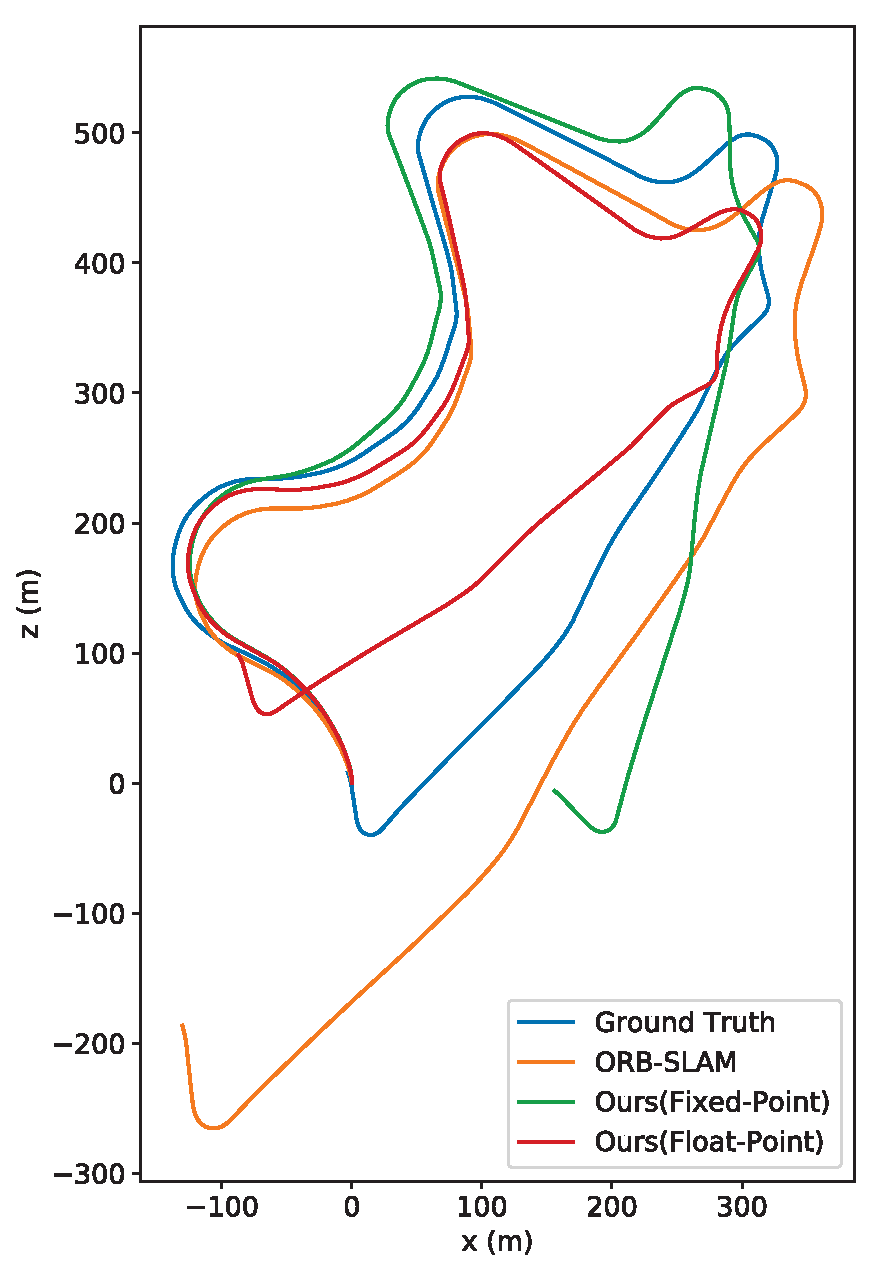
\includegraphics[height=0.9\linewidth]{fig/sequence_09.eps}} 
    \subfigure[Traj. on Seq. 10] {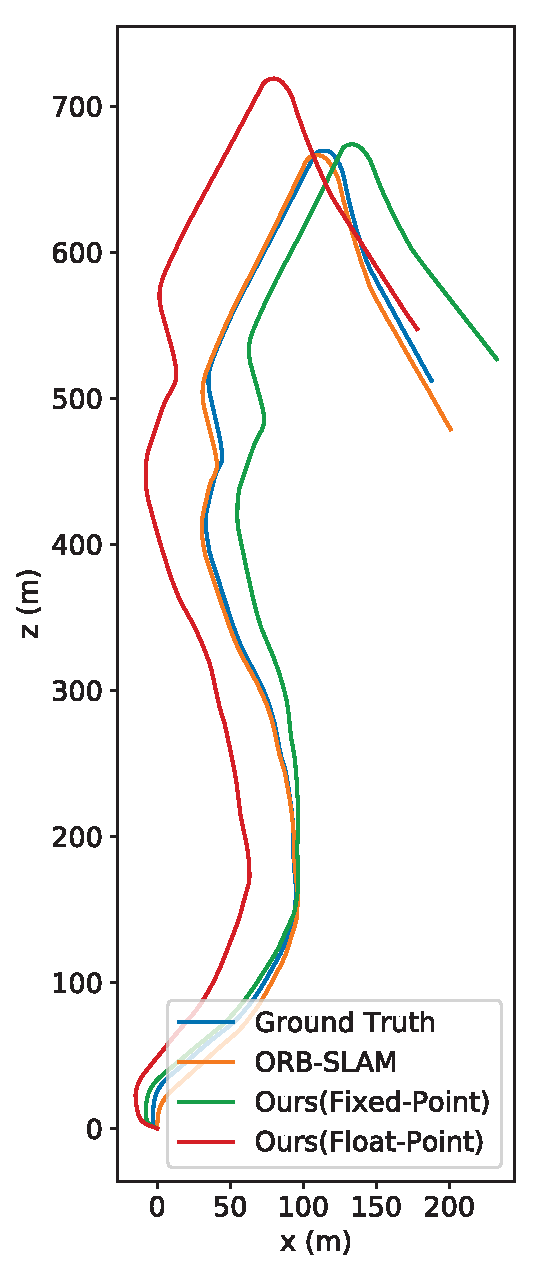
\includegraphics[height=0.9\linewidth]{fig/sequence_10.eps}} 
    \caption{Qualitative evaluation of odometry on the KITTI Odometry test sequences (09, 10).}
    \label{fig:VO}
  \end{figure}


Because of the fixed-point number used in our design, which sacrifices the precision of the CNN, the VO accuracy is not as good as the previous works \cite{Mur-Artal:2017281, Zhan:2018e92}. On the other hand, our VO can calculate the 6-D pose within $20ms$ on a resource-constrained embedded platform.


\subsection{Run-Time}

We evaluate our DSLAM on two intelligent cars which are controlled by the Deephi Aristotle board with a ZU9 MPSOC. \Cref{tab:time} shows the run time of each part of our DSLAM system. The pipeline of scheduling of these parts is shown in \cref{sec:background}.


% \begin{figure}[t]
%     \centering  
%     \includegraphics[width=0.95\linewidth]{fig/env.eps}
%     \caption{The intelligent car with the Zynq MPSoC board.}
%     \label{fig:env}
% \end{figure}

\begin{table}[h]
    \centering
    \caption{Run-Time of each part in our DSLAM}
    \footnotesize
    \begin{threeparttable}
  % Table generated by Excel2LaTeX from sheet 'Sheet2'
  \setlength{\tabcolsep}{1mm}{
% Table generated by Excel2LaTeX from sheet 'Sheet1'
    \begin{tabular}{|c|c|c|c|c|}
    \hline
          & NetVLAD, PL & VO, PL  & VO, PS  & NetVLAD, PS  \bigstrut[t]\\
          & ($T_{0}$) &  ($T_{1}$) &  ($T_{2}$) &  ($T_{3}$) \bigstrut[b]\\
    \hline
    Execute time & \multirow{2}[2]{*}{66} & \multirow{2}[2]{*}{3} & \multirow{2}[2]{*}{10} & \multirow{2}[2]{*}{354} \bigstrut[t]\\
    (ms)  &       &       &       &  \bigstrut[b]\\
    \hline
    \end{tabular}%
    
  }
  \begin{tablenotes}
        \item[*] We read the camera at 20fps, so the $T_{f}$ in \cref{fig:pipline} is 50ms.
        \end{tablenotes}
      \end{threeparttable}
    \label{tab:time}%
    
  \end{table}%

Substituting the run-time of each part into \cref{equ:pipeline1,equ:pipeline2,equ:pipeline3}. We find out that the run-time of NetVLAD on PS ($T_{3}$) becomes the bottleneck of the system and \cref{equ:pipeline3} constrains the NetVLAD frequency ($N$) to $8$.

We calculate the relative 6-D pose between every two successive frames and the NetVLAD code every $8$ frames in the following experiments.

\subsection{NetVLAD with DPU}

We evaluate the NetVLAD performance on the loop close dataset for KITTI\cite{KITTIGroundTruth}.
The dataset labels the ground truth of loop closure for these sequences based on the metric positions of each image. Specifically, it compares the position of each image to the others in the sequence and regards the one as a loop if it lies within a radius of $6m$.

The precision-recall curves of the original NetVLAD with an output of 4096 dimensions (Blue), fixed-point NetVLAD 4096-D output (Green), original NetVLAD with 128-D output (Red), and fixed-point NetVLAD 128-D output (Yellow) are shown in \cref{fig:reloc}. We use sequence 00 as the test sequence.


\begin{figure}[t]
  \centering  
  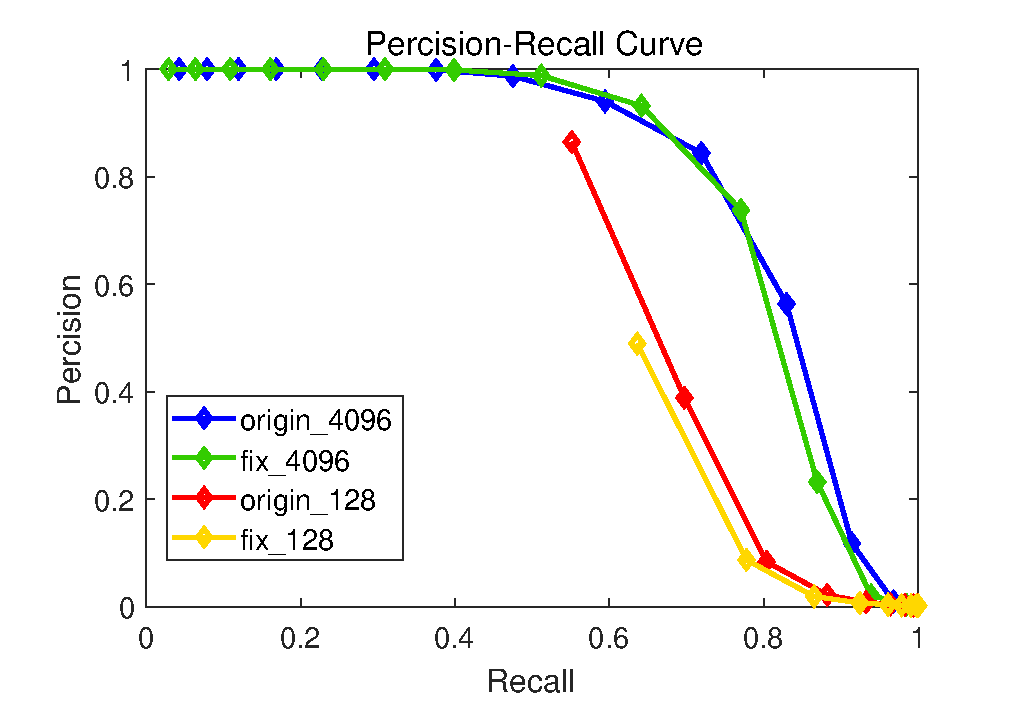
\includegraphics[width=0.75\linewidth]{fig/val_reloc.eps}
  \caption{ROC curves on sequence 00.}
  \label{fig:reloc}
\end{figure}

Our NetVLAD with DPU performs similarly to the original NetVLAD with the same output dimension but runs much faster with the help of the acceleration techniques on FPGA and architecture design. Even if there are sightly accuracy reduction on the ROC curves, the following experiment shows that the slight drawback would not make the overall DSLAM performance decline.

\subsection{DSLAM Evaluation}

With the help of our hardware-software co-design VO and place recognition components on the embedded system, we can build up the DSLAM system like the previous work \cite{Cieslewski:20187ee}. However, unlike the feature point based method in previous \cite{Cieslewski:20187ee}, our approach does not necessarily compute the feature point for each frame. The previous work \cite{Cieslewski:20187ee} transfers the ORB feature points among agents to do inter-robot pose estimation and trajectory merging.

%讲下更具体的实验设计

A possible way to solve the inter-robot pose estimation is to calculate the feature points and descriptors of the corresponding robot and frames when the inter-robot loop closure occurs. However, on the one hand, the traditional feature point detection and description method cannot get the absolute scale from a single image. On the other hand, it is resource consuming to do feature point algorithms like SIFT\cite{Jegou:2010f45} and ORB\cite{Mur-Artal:2017281}. The agents may stop and solve the feature points. We directly transfer the down-sampled $608 \times 160$ image among the agents and use the same method as the proposed VO with DPU to do the inter-robot pose estimation. The result of the merged trajectory is illustrated in \cref{fig:dslam}.


\begin{figure}[ht]
  \centering  
  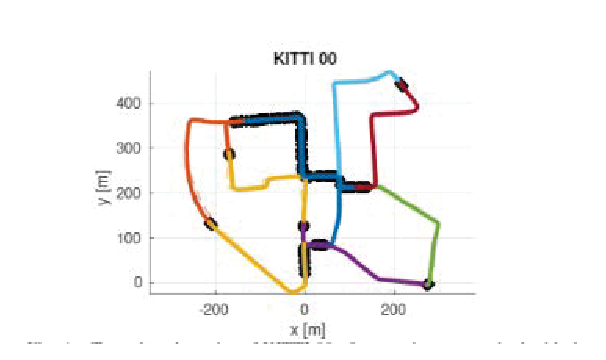
\includegraphics[width=0.85\linewidth]{fig/dslam.eps}
  \caption{??? The sub-trajectory of each agent and the merged trajectory.}
  \label{fig:dslam}
\end{figure}

\begin{figure}[thb]
  \centering  
  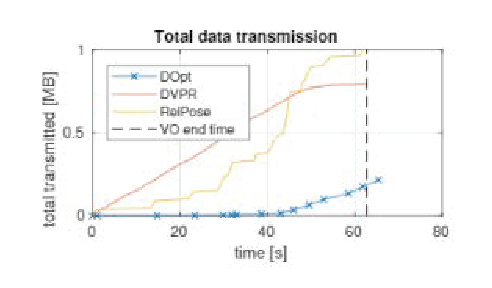
\includegraphics[width=0.85\linewidth]{fig/data.eps}
  \caption{??? The total communication traffic of the propsoed DSLAM}
  \label{fig:data}
\end{figure}

There are three kinds of data need to be transferred among the agents and the server: $1)$ the VO results of each frame (VO), $2)$ the NetVLAD results of every $8$ frames (NetVLAD), $3)$ the image need for inter-robot relative pose estimation (RelPose).

At the beginning of the task, there is no inter-robot loop closure detected, so there is no data traffic for RelPose. When inter-robot loop closure occurs, the data traffic for RelPose increases rapidly. The previous work\cite{Cieslewski:20187ee} also faces this problem though it uses feature point for inter-robot relative pose estimation.


The total communication traffic of the proposed DSLAM system on KITTI 00 is increasing with time and is shown in \cref{fig:data}.
